\chapter{光与物质的相互作用}
\section{光谱}
通过恒星光谱的多普勒频移可以计算恒星的视向速度(式\ref{eq:doppler})。

现代天文学家使用光谱仪来获取恒星的光谱,光谱的作用是把接收到的恒星的复合光按照不同波长展开,目前大多使用衍射光栅来实现。

越好的光谱仪能够将光谱展的越开,展现更加精细的光谱结构,因此定义光谱仪的分辨本领:
\begin{equation}
  \Delta\lambda={\lambda \over nN}
\end{equation}

\paragraph{基尔霍夫定律}\label{kirchhoffs}
\begin{itemize}
  \item 一团热的稠密气体或固体能够产生没有暗线的连续光谱
  \item 一团热的稀薄气体能够产生明亮的光谱线(发射线),发射线频率与跃迁的能级差对应
  \item 一团冷的稠密气体挡在一个产生连续光谱的光源前,能够在连续谱上产生对应原子能级的暗线(吸收线),吸收线频率与跃迁的能级差对应
\end{itemize}

基尔霍夫定律中的\textbf{冷}与\textbf{热}都是相对而言。

\section{光子}
\paragraph{光电效应}
当光照射在金属表面,会从金属表面激发出电子的过程

由于存在原子能级,只有频率大于\textbf{截止频率}的光子才能够激发出电子,在激发出电子的基础上,增加光强只能增加激发出的电子数目,增加入射光的频率能够增加电子的出射动能:
\begin{equation}
  K_\mathrm{max}=E_\mathrm{photon}-\underbrace{\phi}_\text{\clap{金属的溢出功(电子的最小结合能)}}=h\upsilon-\phi={hc \over \lambda}-\phi
\end{equation}

\paragraph{康普顿效应}
高能光子与自由电子发生碰撞,散射光子能量降低的过程,如图\ref{fig:compton}。

\begin{figure}[hbt]
  \centering
  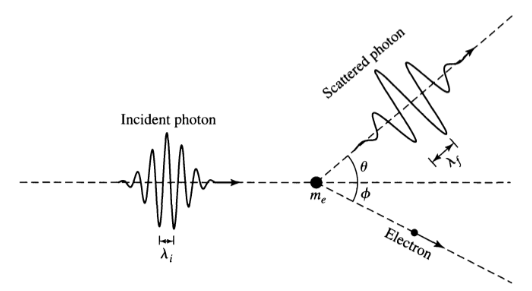
\includegraphics[width=10cm]{chapters/05/compton}
  \caption{康普顿散射示意图}
  \label{fig:compton}
\end{figure}

\section{玻尔的原子模型}
玻尔的原子模型指出,\textbf{原子核周围存在不同的轨道能级,电子位于固定能级上,能级跃迁需要吸收或释放相应能量(光子)},如图\ref{fig:atom}。

通过假设原子核与电子通过库仑力相互作用,以及角动量量子化,得到代表轨道半径的\textbf{玻尔半径}:
\begin{equation}
  r_n={4\pi \epsilon_0 \hbar^2 \over \mu e^2}n^2=a_0n^2
\end{equation}

以及轨道能级:
\begin{equation}
  E_n=-{\mu e^4\over 32\pi^2\epsilon^2\hbar^2}{1\over n^2}=-13.6\;\mathrm{eV}{1\over n^2}
\end{equation}

其中$n$为主量子数,表征原子的每个轨道。

\begin{figure}
  \centering
  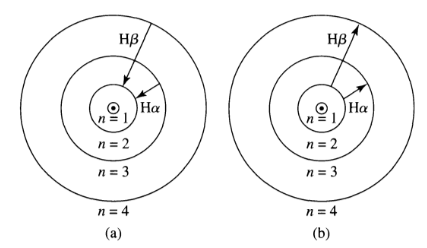
\includegraphics[width=10cm]{chapters/05/atom}
  \caption{玻尔的氢原子模型的巴尔末线系(a)发射线(b)吸收线}
  \label{fig:atom}
\end{figure}

玻尔的模型能够较好的解释实验得到的氢原子发射谱线,并可以计算得到氢原子的基态能量$E_1=-13.6\;\mathrm{eV}$,通过计算不同能级的能量差,可以得到轨道跃迁对应的光子波长:
\begin{equation}
  E_\mathrm{photon}=E_\mathrm{high}-E_\mathrm{low}\notag
\end{equation}

或写为
\begin{equation}
  {hc \over \lambda}=-{\mu e^4\over 32\pi^2\epsilon^2\hbar^2} \left({1\over n_\mathrm{high}^2}- {1\over n_\mathrm{low}^2}\right)
\end{equation}

电子在$n=1$与更高能级的相互跃迁所产生的一系列谱线称为\textbf{莱曼线系},用符号Ly表示,$n=1$和$n=2$之间跃迁为Ly$\alpha$,$n=1$和$n=3$之间跃迁为Ly$\beta$,以此类推。

同理,电子在$n=2$与更高能级的相互跃迁所产生的一系列谱线称为\textbf{巴尔末线系},图\ref{fig:atom}所示为波尔模型的氢原子的巴尔末线系,用符号H表示,$n=2$和$n=3$之间跃迁为H$\alpha$,$n=2$和$n=4$之间跃迁为H$\beta$,以此类推。其他线系如图\ref{fig:level}

\begin{figure}[hbt]
  \centering
  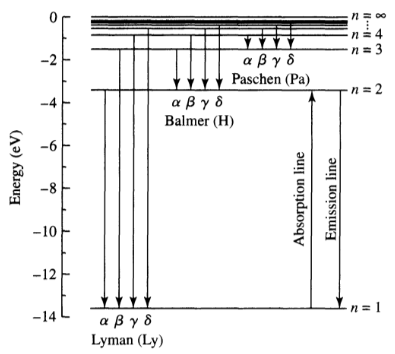
\includegraphics[width=7cm]{chapters/05/level}
  \caption{氢原子的能级跃迁图,包括莱曼、巴尔末、帕邢线系}
  \label{fig:level}
\end{figure}

\section{量子力学}
\subsection{物质波}
德布罗意将\textbf{波粒二象性}推广到所有粒子,提出了物质波,并给出了相应的波长和频率的表达式:
\begin{align}
  \upsilon &= {E\over h}\\[2mm]
  \lambda &= {h\over p}
\end{align}

这种波长和频率被称为德布罗意波长和频率,实际上该式可以推广到一切物体,如计算得到\textbf{一个慢跑的人类的德布罗意波长}$\lambda\sim3.16\times10^{-36}\;\mathrm m$,远小于观测极限,因此可以忽略不计。

\subsection{海森堡的不确定性原理}\label{uncertainty}
不确定性原理指出波粒二象性的内禀属性,当观测时,粒子的位置确定,则动量的不确定会变大,反之亦然。

\begin{equation}
  \Delta x \;\Delta p\geq{1\over2}\hbar
\end{equation}

也可以近似表达为
\begin{equation}
  \Delta x \;\Delta p\approx \hbar
\end{equation}

同时对应能量和时间也存在不确定性关系:
\begin{equation}
  \Delta E \;\Delta t\approx \hbar
\end{equation}

\paragraph{量子隧穿}
由于波粒二象性,粒子以几率波的形式分布在空间中,对于一些比较高的势垒,从能量角度看可能无法穿过,但是实际上波函数已经穿透,只是透过之后很快衰减了。但是波函数透过代表就有一定几率粒子能够穿过势垒,发生量子隧穿。

\subsection{薛定谔方程和量子力学原子模型}
为了描述粒子的波动性,薛定谔提出\textbf{薛定谔方程}来描述波函数,同时发现仅仅通过主量子数$n$无法完全描述原子的能级,提出
\begin{itemize}
  \item \textbf{角量子数}$\ell$,描述原子的角动量$L=\sqrt{l(l+1)}\hbar$,$\ell=0,1,2,3,4,5$等分别对应轨道$s,p,d,f,g,h$等。
  \item \textbf{磁量子数}$m_\ell$,描述原子角动量$z$分量$L_z=m_\ell \hbar$,$m_\ell$为$-\ell$和$+\ell$间的任意整数。
\end{itemize}

不同的轨道量子数$\ell$和$m_\ell$但具有相同的主量子数(相同能量)称为\textbf{简并}。

同时电子还具有\textbf{自旋量子数}$m_s=\pm{1\over2}$,用来表征电子内禀的自旋角动量$z$分量$S_z=m_s \hbar$。

电子由于具有不同的自旋,在磁场中会产生不同的能级,导致谱线会分裂,这种现象称为\textbf{塞曼效应},对于频率为
\begin{equation}
  \upsilon=\upsilon_0\qquad \text{和}\qquad \upsilon_0\pm{eB\over 4\pi\mu}
\end{equation}

\paragraph{泡利不相容原理}
两个电子不能具有完全相同的一组(4个)轨道量子数。

实际上泡利不相容原理适用于所有费米子(电子、中子等构成物质的基本粒子),而玻色子(光子等构成能量的基本粒子)可以具有完全相同的能量状态,且费米子的自旋角动量只能是${1\over2}\hbar$的奇数倍,而玻色子的自旋角动量是$\hbar$的整数倍。